

%-------------------------------------------------------------------------------
% Dokumenten Klasse
\documentclass[
	final,
	a4paper,
	oneside,
	parskip=full,
	headings=standardclasses,
	headings=big,
	pointednumbers
]{scrartcl}

%-------------------------------------------------------------------------------
% Packete nutzen
\usepackage{ngerman,palatino,setspace}
\usepackage[T1]{fontenc}
\usepackage[utf8]{inputenc}
\usepackage[left=20mm,right=20mm,top=25mm,bottom=25mm]{geometry}
\usepackage{amsmath}
\usepackage{mathtools}
\usepackage{tikz}

\usetikzlibrary{automata, positioning, arrows, calc}

%{
%\tikzset{
%    ->, % makes the edges directed
%    >=stealth, % makes the arrow heads bold
%    node distance=2cm, % specifies the minimum distance between two nodes. Change if necessary.
%    every state/.style={thick, fill=gray!10}, % sets the properties for each ’state’ node
%    every edge/.append style={line width=0.25mm}, % sets the properties for each ’state’ node
%    initial text=$ $, % sets the text that appears on the start arrow
%}
%}

\tikzset{
    node distance=2cm, % Minimum distance between two nodes. Change if necessary.
    every state/.style={ % Sets the properties for each state
        semithick,
        fill=gray!10
    },
    initial text={}, % No label on start arrow
    double distance=2pt, % Adjust appearance of accept states
    every edge/.style={ % Sets the properties for each transition
        draw,
        ->,>=stealth, % Makes edges directed with bold arrowheads
        auto,
        semithick
    },
}


\newcommand{\notaccept}[3]{($(#1)+(#2,#2)$)   -- ($(#1)+(#3,#3)$)
    ($(#1)+(-#2,-#2)$) -- ($(#1)+(-#3,-#3)$)
    ($(#1)+(#2,-#2)$)  -- ($(#1)+(#3,-#3)$)
    ($(#1)+(-#2,#2)$)  -- ($(#1)+(-#3,#3)$)}

%-------------------------------------------------------------------------------
% New Font package
%\usepackage{bm}
%\usepackage[sc]{mathpazo}

\def\boldeps{\boldsymbol{\varepsilon}}

%-------------------------------------------------------------------------------
\usepackage{multirow}

%-------------------------------------------------------------------------------
% uline
\usepackage{ulem}

%-------------------------------------------------------------------------------
% Anderer Font
\usepackage{mathrsfs}
\usepackage[mathcal]{euscript}

%-------------------------------------------------------------------------------
% Square brackets
\usepackage{stmaryrd}

%-------------------------------------------------------------------------------
% Better tables
\usepackage{tabularx}
\usepackage{siunitx}
\usepackage{ragged2e}
\usepackage{array}

%-------------------------------------------------------------------------------
% 
\newcommand{\st}[1]{%
    \tikz[baseline=(char.base)]\node[circle, draw=black, inner sep=2pt](char){#1} ;}
\newcommand{\sta}[1]{%
    \tikz[baseline=(char.base)]\node[double, circle, draw=black, inner sep=2pt](char){#1} ;}

\newcommand{\f}[2]{\frac{#1}{#2}}
\newcommand{\e}{\mathrm{e}}
\newcommand{\kl}[1]{{\left( #1 \right)}}
\newcommand{\kq}[1]{{\left\{ #1 \right\}}}
\newcommand{\ks}[1]{{\left[ #1 \right]}}

%-------------------------------------------------------------------------------
% Dokument
\begin{document}
    
    \def\pagein{0.15}
    \def\pageout{0.85}
    
    %--- Page 1 --------------------------------------------------------------------
    
    % --- Sprache A ---

    $\Sigma = \left\{ \; a, b \; \right\} $ \quad
    $R = `` \left( \; ab \cup a \; \right)^* "{} $ \quad
    $\mathscr{L} = \llbracket \; \left( \; ab \cup a \; \right)^* \; \rrbracket $
    
    \begin{minipage}{\pagein\textwidth}
        $a$:
    \end{minipage}
    \begin{minipage}{\pageout\textwidth}
        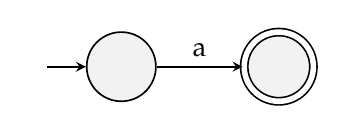
\begin{tikzpicture}
            \node[state, initial left]                  (q1)    {};
            \node[state, accepting, right of=q1]        (q2)    {};
            \draw   (q1) edge[]         node{a} (q2)
            ;
        \end{tikzpicture}
    \end{minipage}
    
    \begin{minipage}{\pagein\textwidth}
        $b$:
    \end{minipage}
    \begin{minipage}{\pageout\textwidth}
        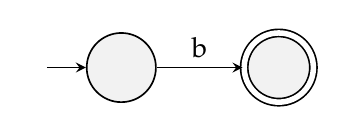
\begin{tikzpicture}
            \node[state, initial left]                  (q1)    {};
            \node[state, accepting, right of=q1]        (q2)    {};
            \draw   (q1) edge[]         node{b} (q2)
            ;
        \end{tikzpicture}
    \end{minipage}
    
    \begin{minipage}{\pagein\textwidth}
        $ab$:
    \end{minipage}
    \begin{minipage}{\pageout\textwidth}
        \def\in{0.25}
        \def\out{0.45}
        \begin{tikzpicture}
            \node[state, initial left]                  (aq1)   {};
            \node[state, accepting, right of=aq1]       (aq2)   {};
            \node[state, right of=aq2]                  (bq1)   {};
            \node[state, accepting, right of=bq1]       (bq2)   {};
            \coordinate (c1) at (aq2);
            \draw   (aq1) edge[]        node{a} (aq2)
                    (bq1) edge[]        node{b} (bq2)
            ;
            \draw[red]
                    \notaccept{c1}{\in}{\out}
                    (aq2) edge[] node{$\boldeps$} (bq1)
            ;
        \end{tikzpicture}
    \end{minipage}
           
    \begin{minipage}{\pagein\textwidth}
       $ab \cup a$:
    \end{minipage}
    \begin{minipage}{\pageout\textwidth}
        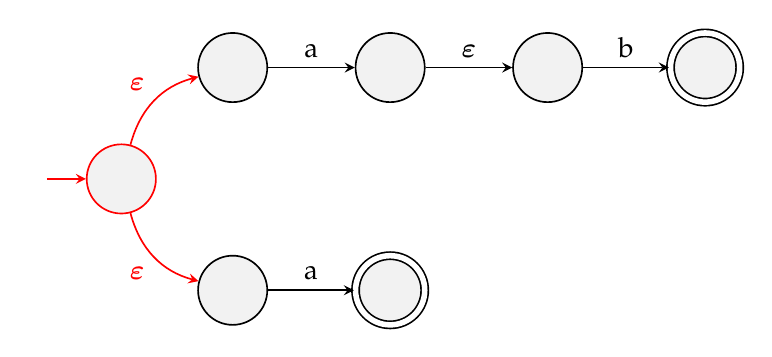
\begin{tikzpicture}[
                every initial by arrow/.style={red}
            ]
            \node[state, initial left, draw=red]                  (aba)   {};
            \node[state, above right of=aba]            (aq1)   {};
            \node[state, right of=aq1]                  (aq2)   {};
            \node[state, right of=aq2]                  (bq1)   {};
            \node[state, accepting, right of=bq1]       (bq2)   {};
            \node[state, below right of=aba]            (aq3)   {};
            \node[state, accepting, right of=aq3]       (aq4)   {};
            \coordinate (x) at (aq2);
            \draw   (aq1) edge[]                        node{a}             (aq2)
                    (bq1) edge[]                        node{b}             (bq2)
                    (aq2) edge[]                        node{$\boldeps$} (bq1)
                    (aq3) edge[]                        node{a}             (aq4)
            ;
            \draw[red, thick]
                    (aba) edge[bend left]               node{$\boldeps$} (aq1)
                    (aba) edge[bend right, below left]  node{$\boldeps$} (aq3)
            ;
        \end{tikzpicture}
    \end{minipage}
           
    \begin{minipage}{\pagein\textwidth}
       $\left(ab \cup a\right)^*$:
    \end{minipage}
    \begin{minipage}{\pageout\textwidth}
        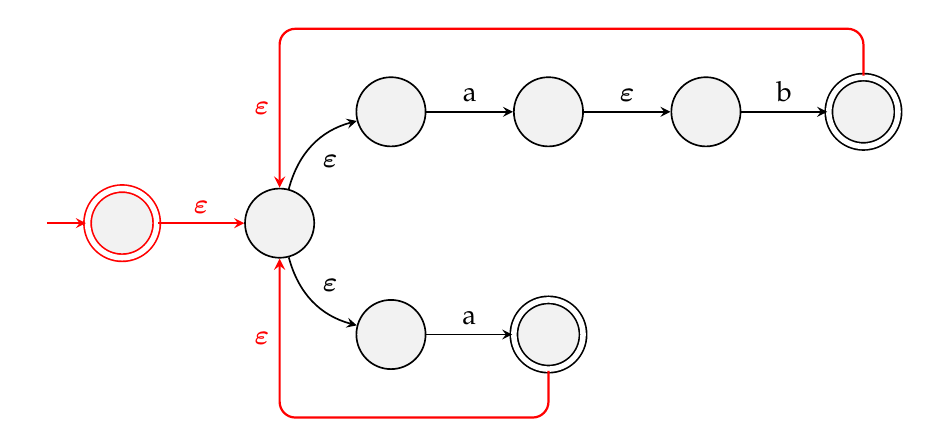
\begin{tikzpicture}[
                every initial by arrow/.style={red}
            ]
            \tikzset{
                rc/.style={->,>=stealth,red,thick,rounded corners=2mm}
            }
            \node[state,initial left,accepting,draw=red](start) {};
            \node[state, right of=start]                (aba)   {};
            \node[state, above right of=aba]            (aq1)   {};
            \node[state, right of=aq1]       (aq2)   {};
            \node[state, right of=aq2]                  (bq1)   {};
            \node[state, accepting, right of=bq1]       (bq2)   {};
            \node[state, below right of=aba]            (aq3)   {};
            \node[state, accepting, right of=aq3]       (aq4)   {};
            \coordinate (x) at (bq2);
            \draw   (aq1) edge[]                        node{a}             (aq2)
                    (bq1) edge[]                        node{b}             (bq2)
                    (aq2) edge[]                        node{$\boldeps$}    (bq1)
                    (aq3) edge[]                        node{a}             (aq4)
                    (aba) edge[bend left,  below right] node{$\boldeps$}    (aq1)
                    (aba) edge[bend right, above right] node{$\boldeps$}    (aq3)
            ;
            %\draw[step=1cm,gray,very thin]
            %        (0, -3) grid (10,3);
            %;
            \draw[red]
                    (start) edge[]                      node{$\boldeps$}    (aba);

            \draw[rc]
                    let \p1 = (bq2),
                        \p2 = (aba)
                    in
                    (bq2) -- (\x1, \y1+30) -- (\x2,\y1+30) -- node[left]{$\boldeps$} (aba);
            \draw[rc]
                    let \p1 = (aq4),
                        \p2 = (aba)
                    in
                    (aq4) -- (\x1, \y1-30) -- (\x2,\y1-30) -- node[left]{$\boldeps$} (aba);
                    
            ;
            %\draw[->,>=stealth,red,thick]
            %        (bq2) .. controls (8,3)
            %                    and      (1,4) ..   node[yshift=-0.3cm]{$\boldeps$} (aba)
            %        (aq4) .. controls (5,-3)
            %                    and      (1,-3) ..  node[yshift=0.3cm]{$\boldeps$} (aba)
            %;
        \end{tikzpicture}
    \end{minipage}

    \quad
    
    \quad

    % --- Sprache B ---
    
    $\Sigma = \left\{ \; 0, 1 \; \right\} $ \quad
    $R = `` \left( \; 0 \cup 1 \; \right)^* 10 "{} $ \quad
    $\mathscr{L} = \llbracket \; \left( \; 0 \cup 1 \; \right)^* 10 \; \rrbracket $
           
    \begin{minipage}{\pagein\textwidth}
       $\left( \; 0 \cup 1 \; \right)^* 10$:
    \end{minipage}
    \begin{minipage}{\pageout\textwidth}
        \def\in{0.25}
        \def\out{0.45}
        \begin{tikzpicture}
            \tikzset{
                rc/.style={->,>=stealth,thick,rounded corners=2mm}
            }
            \node[state,initial left,accepting]         (start) {};
            \node[state, right of=start]                (01)    {};
            % oben
            \node[state, above right of=01]             (0q1)   {};
            \node[state, accepting, right of=0q1]       (0q2)   {};
            % unten
            \node[state, below right of=01]             (1q1)   {};
            \node[state, accepting, right of=1q1]       (1q2)   {};
            % rechts
            \node[state, below right of=0q2]            (r1q1)  {};
            \node[state, accepting, right of=r1q1]      (r1q2)  {};
            \node[state, right of=r1q2]                 (r0q1)  {};
            \node[state, accepting, right of=r0q1]      (r0q2)  {};
            
            \coordinate (c1) at (0q2);
            \coordinate (c2) at (1q2);
            \coordinate (c3) at (r1q2);
            \draw   (0q1) edge[]                        node{0}             (0q2)
                    (1q1) edge[]                        node{1}             (1q2)
                    (01) edge[bend left,  below right]  node{$\boldeps$}    (0q1)
                    (01) edge[bend right, above right]  node{$\boldeps$}    (1q1)
                    (start) edge[]                      node{$\boldeps$}    (aba)
                    (0q2) edge[bend left, below left]   node{$\boldeps$}    (r1q1)
                    (1q2) edge[bend right, above left]  node{$\boldeps$}    (r1q1)
                    (r1q1) edge[]                       node{1}             (r1q2)
                    (r1q2) edge[]                       node{$\boldeps$}    (r0q1)
                    (r0q1) edge[]                       node{0}             (r0q2)
            ;

            \draw[rc]
                    let \p1 = (0q2),
                        \p2 = (01)
                    in
                    (0q2) -- (\x1, \y1+22) -- (\x2,\y1+22) -- node[left]{$\boldeps$} (01);
            \draw[rc]
                    let \p1 = (1q2),
                        \p2 = (01)
                    in
                    (1q2) -- (\x1, \y1-22) -- (\x2,\y1-22) -- node[left]{$\boldeps$} (01);
            \draw[rc]
                    let \p1 = (start),
                        \p2 = (r1q1)
                    in
                    (start) -- (\x1, \y1-80) -- (\x2,\y1-80) -- node[right]{$\boldeps$} (r1q1);
                    
            ;
            \draw[thick]
                    \notaccept{c1}{\in}{\out}
                    \notaccept{c2}{\in}{\out}
                    \notaccept{c3}{\in}{\out}
            ;
            %\draw[->,>=stealth,red,thick]
            %        (bq2) .. controls (8,3)
            %                    and      (1,4) ..   node[yshift=-0.3cm]{$\boldeps$} (aba)
            %        (aq4) .. controls (5,-3)
            %                    and      (1,-3) ..  node[yshift=0.3cm]{$\boldeps$} (aba)
            %;
        \end{tikzpicture}
    \end{minipage}
    
    %--- Page 2 --------------------------------------------------------------------
    \newpage    

    \textbf{Syntax und Semantik von regulären Ausdrücken (Regular Expression, RE)}

    Sei $R$ ein $RE$. Dann $\mathscr{L} \llbracket R \rrbracket $ ist die Sprache,
    die von $R$ beschrieben wird.

    %\renewcommand\tabularxcolumn[1]{m{#1}}
    %\setlength{\extrarowheight}{0.3cm}
    %\newcolumntype{b}{l}
    %\newcolumntype{s}{l}
    \renewcommand{\arraystretch}{1.5}
    \begin{tabular}{l|l|l}
        \multicolumn{1}{l}{} &
        \multicolumn{1}{l}{$R$ (Syntax)} &
        \multicolumn{1}{l}{$\mathscr{L} \llbracket R \rrbracket$ (Semantik)} \\
        \hline
        1) & $a$ für $a \in \Sigma$                         & $\left\{ a \right\}$ \\
        2) & $\emptyset$ (kein Zeichen)                     & $\emptyset$ \\
        3) & $\varepsilon$ (leeres Wort)                    & $\left\{ \varepsilon \right\}$ \\
        \hline
        4) & $\left(R_1 \cup R_2\right)$                    & $\mathscr{L} \llbracket R_1 \rrbracket \cup
                                                               \mathscr{L} \llbracket R_2 \rrbracket$ \\
        5) & $\left(R_1 \cdot R_2\right)$                   & $\mathscr{L} \llbracket R_1 \rrbracket \cdot
                                                               \mathscr{L} \llbracket R_2 \rrbracket$ \\
        6) & $\left(R^*\right)$                             & $\left( \mathscr{L} \llbracket R_1
                                                              \rrbracket \right)^*$
    \end{tabular}
    
    

    %--- Page 3 --------------------------------------------------------------------
    \newpage

    $ 0 \quad 0^* \quad 1 \quad 10^*10^* \quad \kl{10^*10^*}^* \quad 0^*\kl{10^*10^*}^* $

    \begin{minipage}{\textwidth}
        \def\in{0.12}
        \def\out{0.27}
        \def\inb{0.17}
        \def\outb{0.32}
        \def\spa{20}
        \def\spb{35}
        \def\spc{50}
        \begin{tikzpicture}[]
            \tikzset{
                rc/.style={->,>=stealth,thick,rounded corners=2mm},
                every state/.style={ % Sets the properties for each state
                    semithick,
                    fill=gray!10,
                    inner sep=2pt,
                    minimum size=2pt
                },
                node distance=1.25cm
            }
            \node[state, accepting,     initial left]   (q1)    {1};
            \node[state,                right of=q1]    (q2)    {2};
            \node[state, accepting,     right of=q2]    (q3)    {3};
            \node[state, accepting,     right of=q3]    (q4)    {4};
            \node[state,                right of=q4]    (q5)    {5};
            \node[state, accepting,     right of=q5]    (q6)    {6};
            \node[state, accepting,     right of=q6]    (q7)    {7};
            \node[state,                right of=q7]    (q8)    {8};
            \node[state, accepting,     right of=q8]    (q9)    {9};
            \node[state,                right of=q9]    (q10)   {10};
            \node[state, accepting,     right of=q10]   (q11)   {11};
            \node[state, accepting,     right of=q11]   (q12)   {12};
            \node[state,                right of=q12]   (q13)   {13};
            \node[state, accepting,     right of=q13]   (q14)   {14};
            
            \coordinate (c1)    at (q1);
            \coordinate (c3)    at (q3);
            \coordinate (c6)    at (q6);
            \coordinate (c7)    at (q7);
            \coordinate (c9)    at (q9);
            \coordinate (c11)   at (q11);
            \draw   (q1)    edge    node{$\boldeps$}    (q2)
                    (q2)    edge    node{$0$}             (q3)
                    (q3)    edge    node{$\boldeps$}    (q4)
                    (q4)    edge    node{$\boldeps$}    (q5)
                    (q5)    edge    node{$1$}           (q6)
                    (q6)    edge    node{$\boldeps$}    (q7)
                    (q7)    edge    node{$\boldeps$}    (q8)
                    (q8)    edge    node{$0$}           (q9)
                    (q9)    edge    node{$\boldeps$}    (q10)
                    (q10)   edge    node{$1$}           (q11)
                    (q11)   edge    node{$\boldeps$}    (q12)
                    (q12)   edge    node{$\boldeps$}    (q13)
                    (q13)   edge    node{$0$}           (q14)
            ;

            % Forward
            \draw[rc]
                    let \p1 = (q1),
                        \p2 = (q4)
                    in
                    (q1) -- (\x1, \y1-\spa) -- (\x1+54, \y1-\spa) node[below]{$\boldeps$} -- (\x2,\y1-\spa) -- (q4);
            \draw[rc]
                    let \p1 = (q7),
                        \p2 = (q10)
                    in
                    (q7) -- (\x1, \y1-\spa) -- (\x1+54, \y1-\spa) node[below]{$\boldeps$} -- (\x2,\y1-\spa) -- (q10);
            % Backward
            \draw[rc]
                    let \p1 = (q3),
                        \p2 = (q2)
                    in
                    (q3) -- (\x1, \y1+\spa) -- (\x1-17, \y1+\spa) node[above]{$\boldeps$} -- (\x2,\y1+\spa) -- (q2);
            \draw[rc]
                    let \p1 = (q9),
                        \p2 = (q8)
                    in
                    (q9) -- (\x1, \y1+\spa) -- (\x1-17, \y1+\spa) node[above]{$\boldeps$} -- (\x2,\y1+\spa) -- (q8);
            \draw[rc]
                    let \p1 = (q14),
                        \p2 = (q13)
                    in
                    (q14.100) -- (\x1-5, \y1+\spa) -- (\x1-17, \y1+\spa) node[above]{$\boldeps$} -- (\x2,\y1+\spa) -- (q13);
            \draw[rc]
                    let \p1 = (q14),
                        \p2 = (q5)
                    in
                    (q14.70) -- (\x1+3, \y1+\spc) -- (\x1-195, \y1+\spc) node[above]{$\boldeps$} -- (\x2-4,\y1+\spc) -- (q5.120);
            \draw[rc]
                    let \p1 = (q12),
                        \p2 = (q5)
                    in
                    (q12) -- (\x1, \y1+\spb) -- (\x1-124, \y1+\spb) node[above]{$\boldeps$} -- (\x2+4,\y1+\spb) -- (q5.60);
                    
            \draw[thick]
                    \notaccept{c1}{\in}{\out}
                    \notaccept{c3}{\in}{\out}
                    \notaccept{c6}{\in}{\out}
                    \notaccept{c7}{\in}{\out}
                    \notaccept{c9}{\in}{\out}
                    \notaccept{c11}{\inb}{\outb}
            ;
        \end{tikzpicture}
    \end{minipage}
	

    \begin{minipage}{\textwidth}
        \def\spa{16}
        \def\spb{35}
        \def\spc{50}
        \begin{tikzpicture}[]
            \tikzset{
                rc/.style={thick, densely dashed},
                every state/.style={ % Sets the properties for each state
                    semithick,
                    fill=gray!10,
                    inner sep=2pt,
                    minimum size=2pt
                },
                node distance=1.25cm
            }
            % 1. Line
            \node[state,                initial left]   (q1)    {1};
            \node[state,                right of=q1]    (q2)    {2};
            \node[state,                right of=q2]    (q4)    {4};
            \node[state,                right of=q4]    (q5)    {5};
            % 2. Line
            \node[state,                below of=q2]    (0q3)   {3};
            \node[state,                right of=0q3]   (0q4)   {4};
            \node[state,                right of=0q4]   (0q5)   {5};
            \node[state,                left of=0q3]    (0q2)   {2};
            % 3. Line
            \node[state,                below of=0q5]   (1q6)   {6};
            \node[state,                right of=1q6]   (1q7)   {7};
            \node[state,                right of=1q7]   (1q8)   {8};
            \node[state,                right of=1q8]   (1q10)  {10};
            % 4. Line
            \node[state,                below of=1q10]  (1q11)  {11};
            \node[state, accepting,     right of=1q11]  (1q12)  {12};
            \node[state,                right of=1q12]  (1q13)  {13};
            \node[state,                left of=1q11]   (1q5)  {5};
            
            \draw   
                    % 1. Line
                    (q1)    edge    node{$\boldeps$}    (q2)
                    (q2)    edge    node{$\boldeps$}    (q4)
                    (q4)    edge    node{$\boldeps$}    (q5)
                    % 2. Line
                    (q2)    edge                        (0q3)
                    (0q2)   edge    node{$\boldeps$}    (0q3)
                    (0q3)   edge    node{$\boldeps$}    (0q4)
                    (0q4)   edge    node{$\boldeps$}    (0q5)
                    % 3. Line
                    (0q5)   edge                        (1q6)
                    (1q6)   edge    node{$\boldeps$}    (1q7)
                    (1q7)   edge    node{$\boldeps$}    (1q8)
                    (1q8)   edge    node{$\boldeps$}    (1q10)
                    % 3. Line
                    (1q10)  edge                        (1q11)
                    (1q5)   edge    node{$\boldeps$}    (1q11)
                    (1q11)  edge    node{$\boldeps$}    (1q12)
                    (1q12)  edge    node{$\boldeps$}    (1q13)
            ;
            % 1. Character: 0
            \draw[rc]
                    let \p1 = (q1)
                    in
                    (\x1-30, \y1-\spa) node[left]{$0$} -- (\x1+300,\y1-\spa);
            % 2. Character: 1
            \draw[rc]
                    let \p1 = (q1),
                        \p2 = (0q3)
                    in
                    (\x1-30, \y2-\spa) node[left]{$1$} -- (\x1+300,\y2-\spa);
            % 3. Character: 1
            \draw[rc]
                    let \p1 = (q1),
                        \p2 = (1q6)
                    in
                    (\x1-30, \y2-\spa) node[left]{$1$} -- (\x1+300,\y2-\spa);

        \end{tikzpicture}

        \renewcommand{\arraystretch}{1.75}
        \begin{tabular}{cl|cl|cl}
            \multicolumn{1}{l}{} &
            \multicolumn{1}{l}{} &
            \multicolumn{1}{l}{} &
            \multicolumn{1}{c}{$0$} &
            \multicolumn{1}{l}{} &
            \multicolumn{1}{c}{$1$} \\
            \hline
            \sta{A} & $1\;2\;4\;5$    & \st{B} & $2\;3\;4\;5$   & \st{C} & $6\;7\;8\;10$    \\
            \sta{B} & $2\;3\;4\;5$    & \st{B} & $2\;3\;4\;5$   & \st{C} & $6\;7\;8\;10$    \\
            \st{C}  & $6\;7\;8\;10$   & \st{D} & $8\;9\;10$     & \st{E} & $5\;11\;12\;13$  \\
            \st{D}  & $8\;9\;10$      & \st{D} & $8\;9\;10$     & \st{E} & $5\;11\;12\;13$  \\
            \sta{E} & $5\;11\;12\;13$ & \st{F} & $5\;13\;14$    & \st{C} & $6\;7\;8\;10$    \\
            \sta{F} & $5\;13\;14$     & \st{F} & $5\;13\;14$    & \st{C} & $6\;7\;8\;10$    
        \end{tabular}
    \end{minipage}

    \begin{minipage}{\textwidth}
        \def\in{0.12}
        \def\out{0.27}
        \def\inb{0.17}
        \def\outb{0.32}
        \def\spa{20}
        \def\spb{35}
        \def\spc{50}
        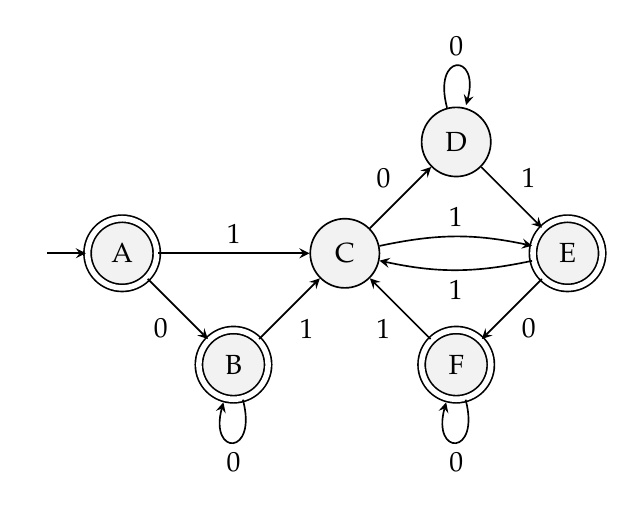
\begin{tikzpicture}[]
            \tikzset{
                rc/.style={->,>=stealth,thick,rounded corners=2mm},
                every edge/.append style={
                    bend angle=12
                }
            }
            \node[state, accepting,     initial left]   (A)     {A};
            \node[state, accepting, below right of=A]   (B)     {B};
            \node[state,            above right of=B]   (C)     {C};
            \node[state,            above right of=C]   (D)     {D};
            \node[state, accepting, below right of=C]   (F)     {F};
            \node[state, accepting, below right of=D]   (E)     {E};
            
            \draw   (A)     edge                node{1}     (C)
                    (A)     edge[below left]    node{0}     (B)
                    (B)     edge[loop below]    node{0}     ()
                    (B)     edge[below right]   node{1}     (C)
                    (C)     edge                node{0}     (D)
                    (C)     edge[bend left]     node{1}     (E)
                    (D)     edge[loop above]    node{0}     ()
                    (D)     edge                node{1}     (E)
                    (E)     edge[bend left]     node{1}     (C)
                    (E)     edge                node{0}     (F)
                    (F)     edge[]              node{1}     (C)
                    (F)     edge[loop below]    node{0}     ()
            ;
        \end{tikzpicture}
    \end{minipage}
    %--- Page 4 --------------------------------------------------------------------
    \newpage
    


    %--- Page 5 --------------------------------------------------------------------
    \newpage
    
    

    %--- Page 6 --------------------------------------------------------------------
    \newpage


\end{document}
